\thispagestyle{fancy}
\justifying
\chapter{Untersuchung des MQW-Designs von AlGaN-UVC-Heterostrukturen}
\label{chap:mqw}
\section{Einleitung}
Dieses Kapitel widmet sich der Untersuchung von AlGaN-MQWs von UVC-LED-Heterostrukturen verschiedener Dicken mit dotierten und undotierten Barrieren. Mit Hilfe der UV-Photolumineszenz sollen der Einfluss der variierenden QW-Dicke und Dotierung auf die interne Quanteneffizienz und die Emissionsenergien untersucht werden. 
\begin{figure}[H]
  \centering
  \begin{minipage}[t]{0.45\textwidth}
    \centering
    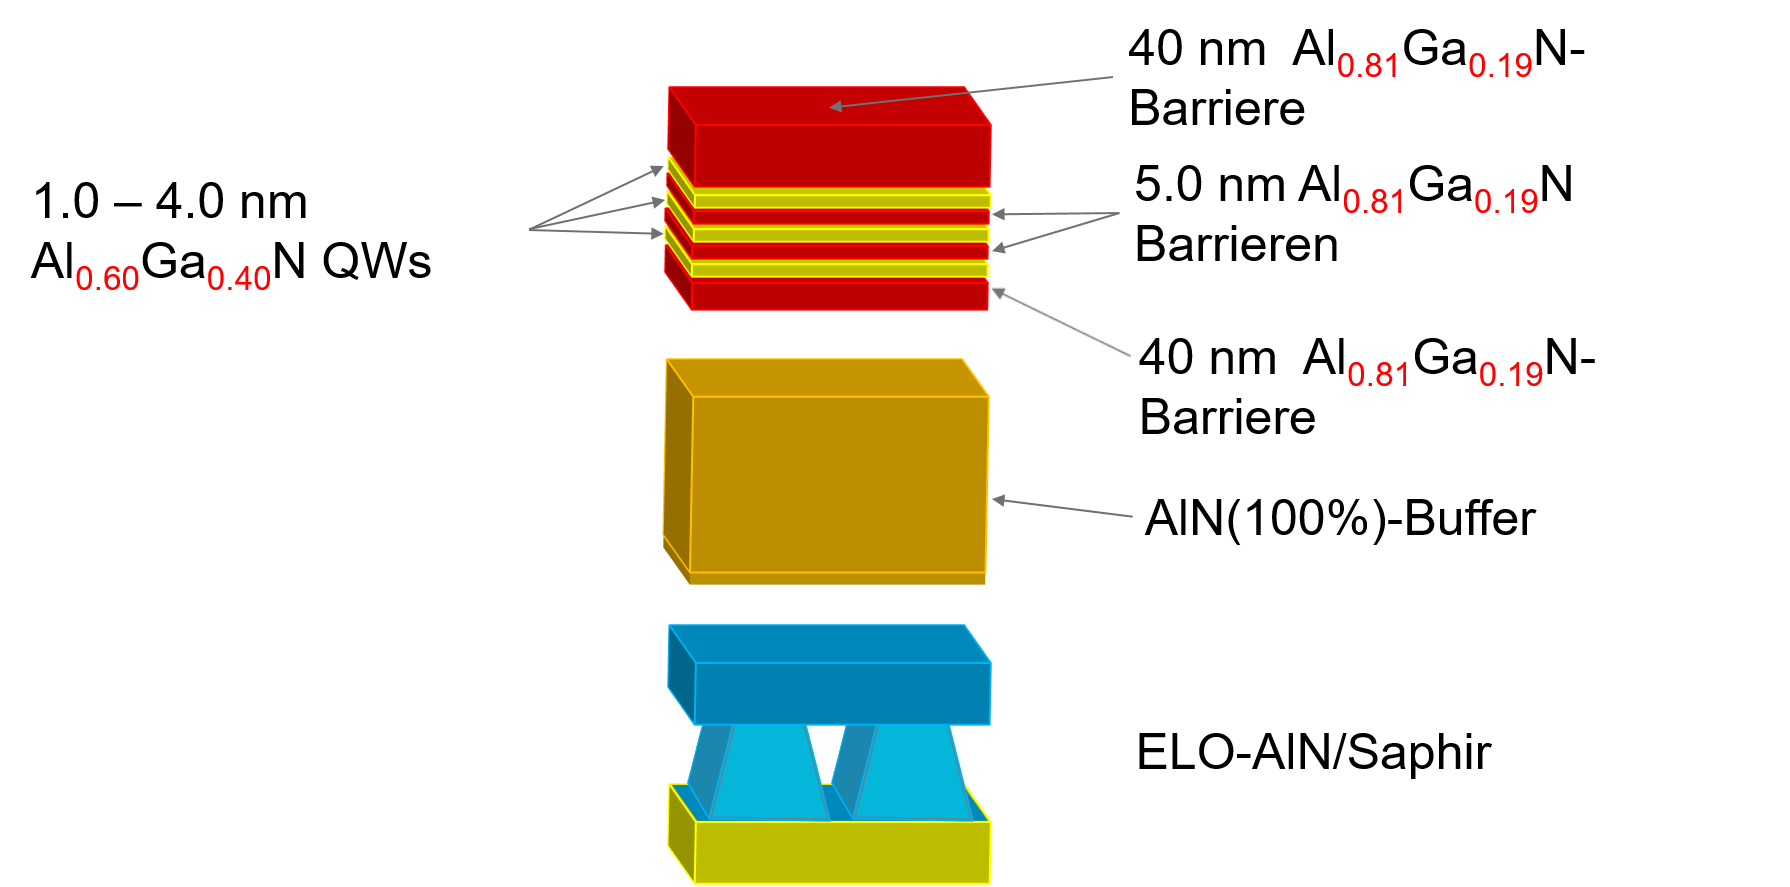
\includegraphics[width=\textwidth]{Bilder/MQWdickenSerie/undotiert}
		\caption{Aufbau der untersuchten MQW-Proben ohne dotierte Barrieren.}
    \label{fig:undotiert}
  \end{minipage}
	\hfill
  \begin{minipage}[t]{0.45\textwidth}
    \centering
    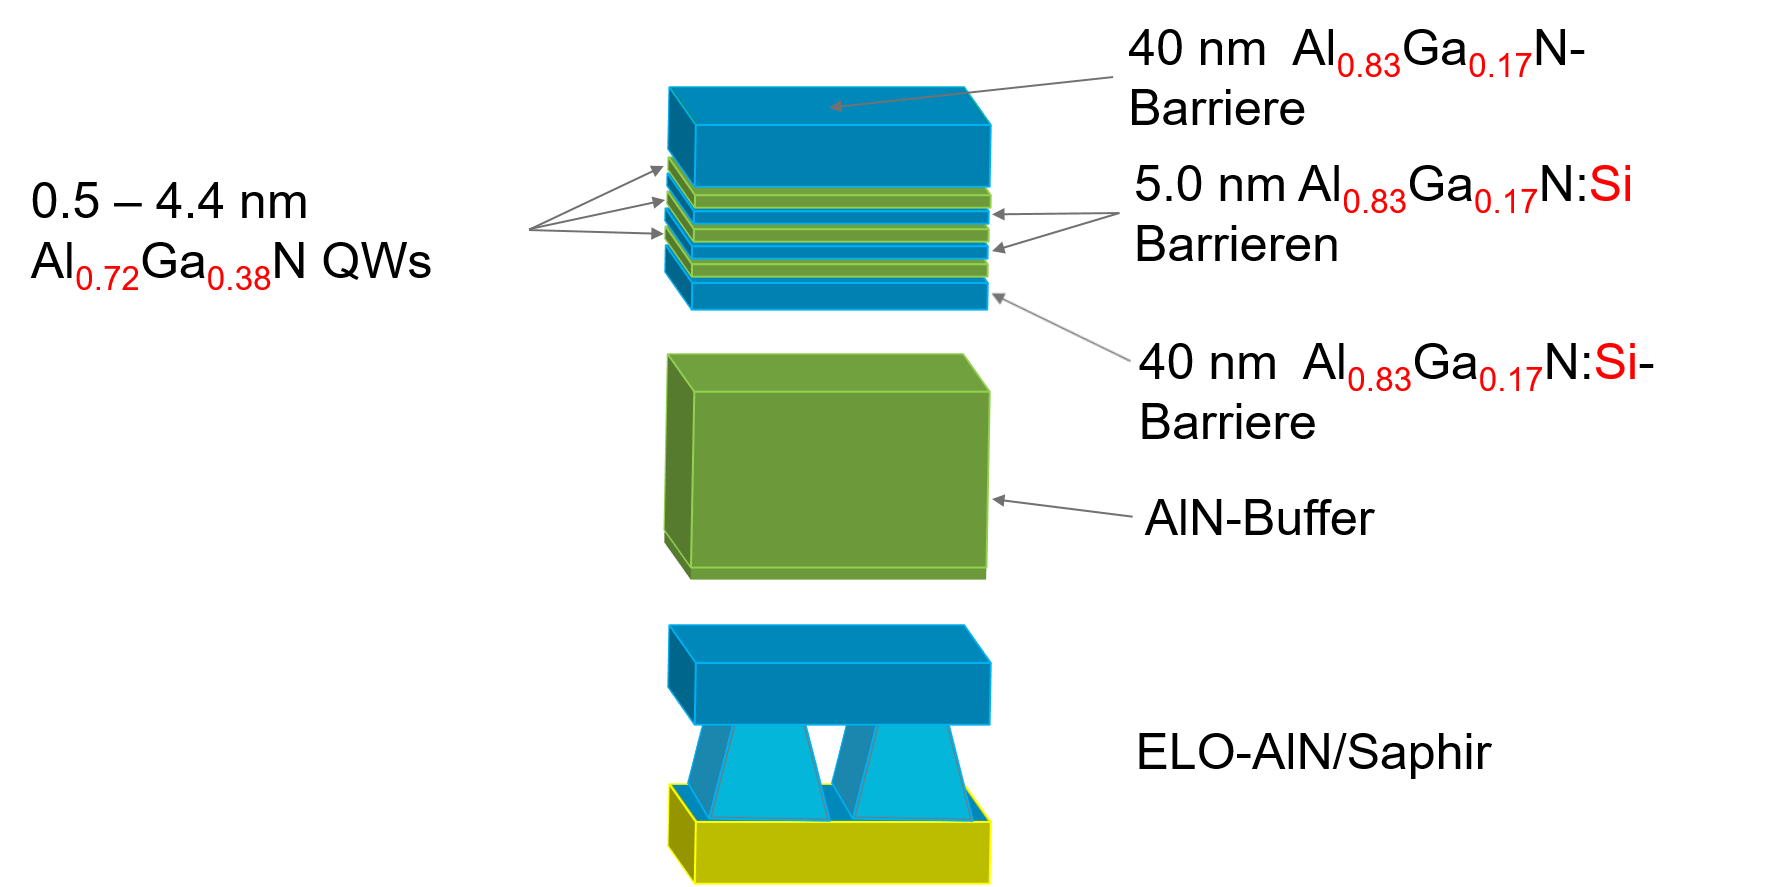
\includegraphics[width=\linewidth]{Bilder/MQWdickenSerie/dotiert}
		\caption{Aufbau der untersuchten MQW-Proben mit dotierten Barrieren.}
    \label{fig:dotiert}
  \end{minipage}
\end{figure}
\noindent 
Der Aufbau der Proben ohne dotierte Barrieren ist in Abbildung \ref{fig:undotiert} zu sehen.
Die aktive Zone setzt sich aus zwei $5 \thinspace nm$ dicken $ Al_{0.81}Ga_{0.19}N$-Barrieren zwischen den drei $ Al_{0.60}Ga_{0.40}N$ QWs mit variierender Dicke $d$ mit $d=1,2,3,4 \thinspace nm$. Die aktive Zone befindet sich zwischen zwei $40 \thinspace nm$ dicken $ Al_{0.81}Ga_{0.19}N$-Barrieren von der eine die oberste Schicht darstellt. Darunter folgt eine AlN ($100\%$)-Bufferschicht die auf einem ELO-AlN/Saphir Substrat aufgewachsen wurde. 
\newline
Abbildung \ref{fig:dotiert} zeigt den Aufbau der Proben mit dotierten Barrieren. Die aktive Zone setzt sich aus zwei $5$nm dicken und Si-dotierten $ Al_{0.83}Ga_{0.17}N:Si$-Barrieren zwischen den drei $ Al_{0.72}Ga_{0.36}N$ QWs mit variierender Dicke $d$ mit $d=0.5,1.0,2.2,4 \thinspace nm$. Die aktive Zone befindet sich zwischen zwei $40 \thinspace nm$ dicken und Si-dotierten $ Al_{0.81}Ga_{0.19}N:Si$-Barrieren von der eine die oberste Schicht darstellt. Darunter folgt eine AlN ($100\%$)-Bufferschicht die auf einem ELO-AlN/Saphir Substrat aufgewachsen wurde. 
\section{Ergebnisse}
Für die experimentelle Untersuchung wurden Photolumineszenzmessungen bei Tieftemperatur gemacht und die Spektren aufgenommen.
In den Spektren, die die Abbildungen \ref{fig:undotiertSpektrumn} und \ref{fig:dotiertSpektrumn} zeigen,
ist deutlich zu erkennen, dass mit sinkender QW-Dicke $d$ die Emissionsenergie steigt.
\begin{figure}[H]
  \centering
  \begin{minipage}[t]{0.45\textwidth}
    \centering
    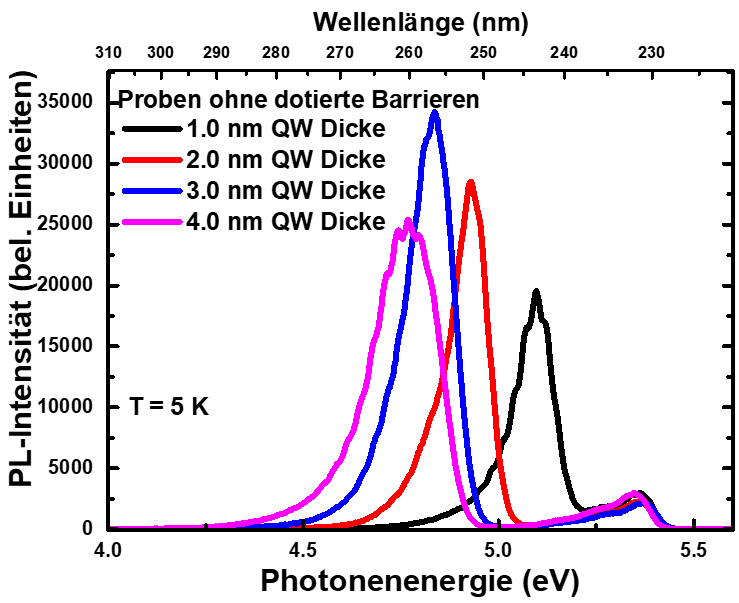
\includegraphics[width=\textwidth]{Bilder/MQWdickenSerie/spektrumUndotiert}
		\caption{PL-Spektren der untersuchten MQW-Proben ohne dotierte Barrieren.}
    \label{fig:undotiertSpektrumn}
  \end{minipage}
	\hfill
  \begin{minipage}[t]{0.45\textwidth}
    \centering
    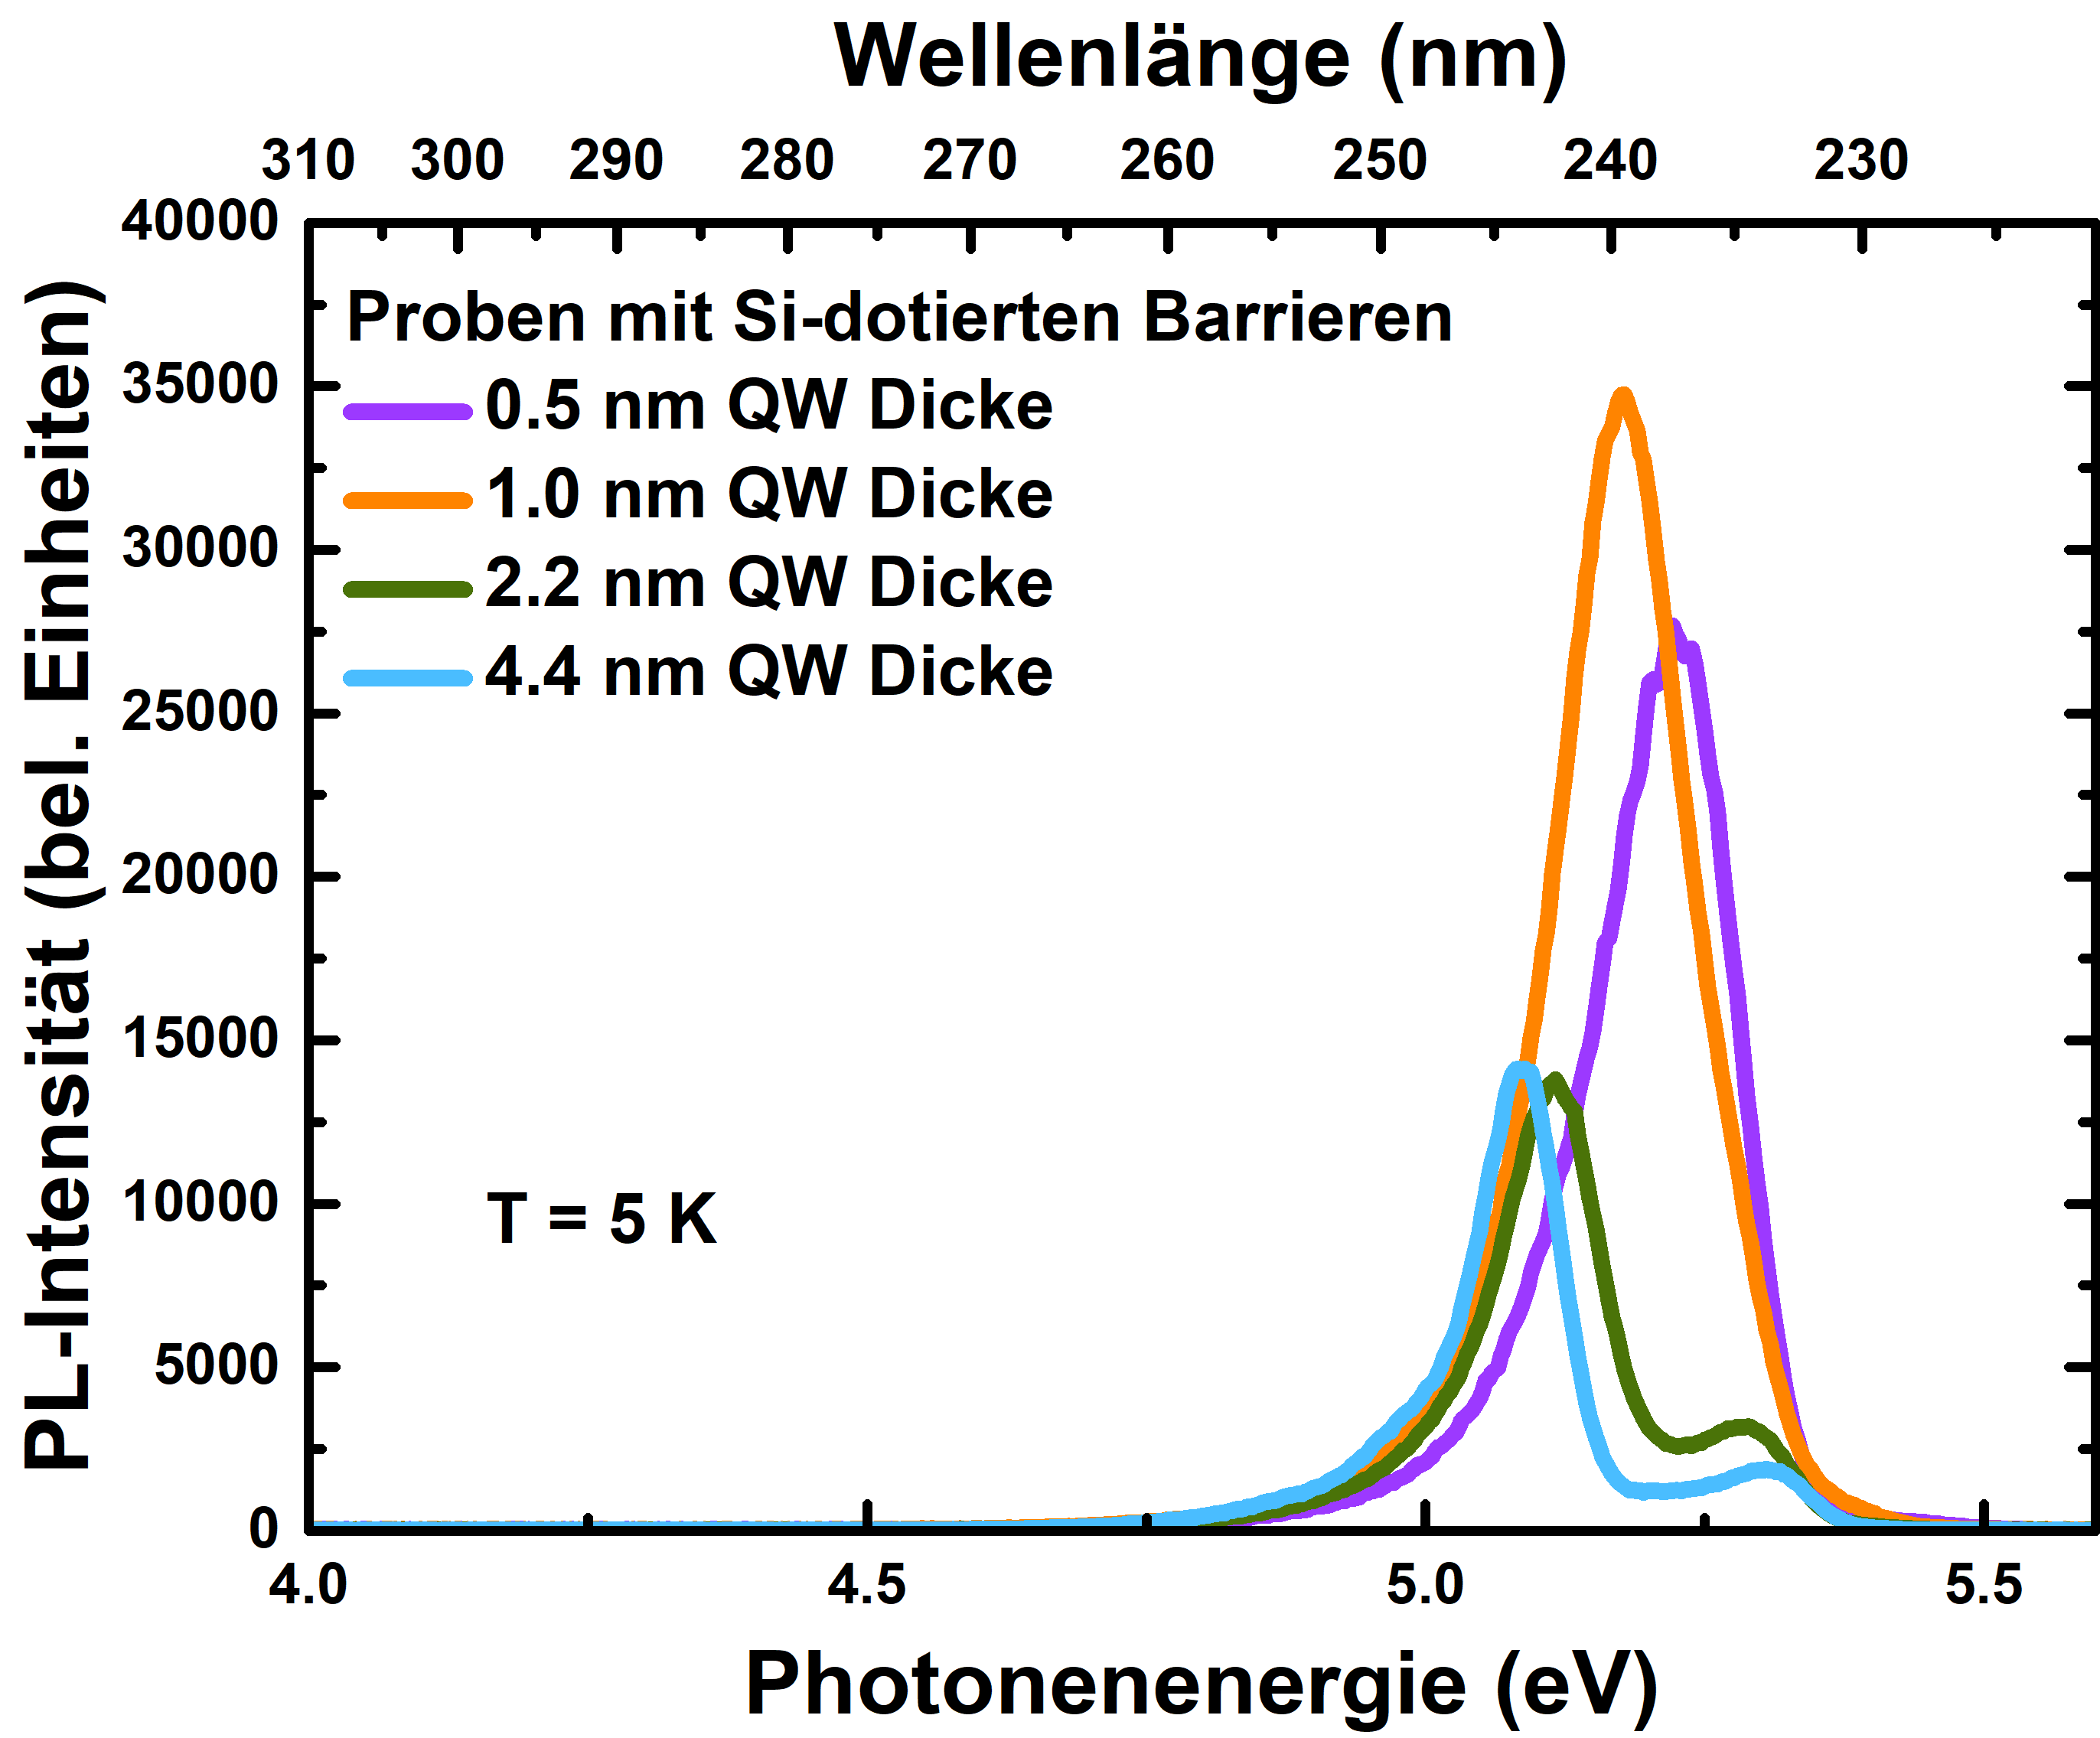
\includegraphics[width=\linewidth]{Bilder/MQWdickenSerie/spektrumDotiert}
		\caption{PL-Spektren der untersuchten MQW-Proben mit dotierten Barrieren.}
    \label{fig:dotiertSpektrumn}
  \end{minipage}
\end{figure}
\noindent 
Die Gründe hierfür sind die Übergangsenergien die mit steigender QW-Dicke \cite{doi:10.1063/1.371241} sinken. 
Die Emissionsenergien fallen im Vergleich deutlich unterschiedlich aus, da die aktiven Zonen beider Serien unterschiedliche Zusammensetzungen (siehe Abb. \ref{fig:undotiert} und \ref{fig:dotiert}) haben. 
\newline
In den Abbildungen \ref{fig:undotiertint} und \ref{fig:dotiertint} ist die integrierte Intensität in Abhängigkeit der Anregungsleistungsdichte bei Tieftemperatur für die Proben mit undotierter und dotierter Barriere in doppeltlogarithmischer Darstellung dargestellt.
\begin{figure}[H]
  \centering
  \begin{minipage}[t]{0.49\textwidth}
    \centering
    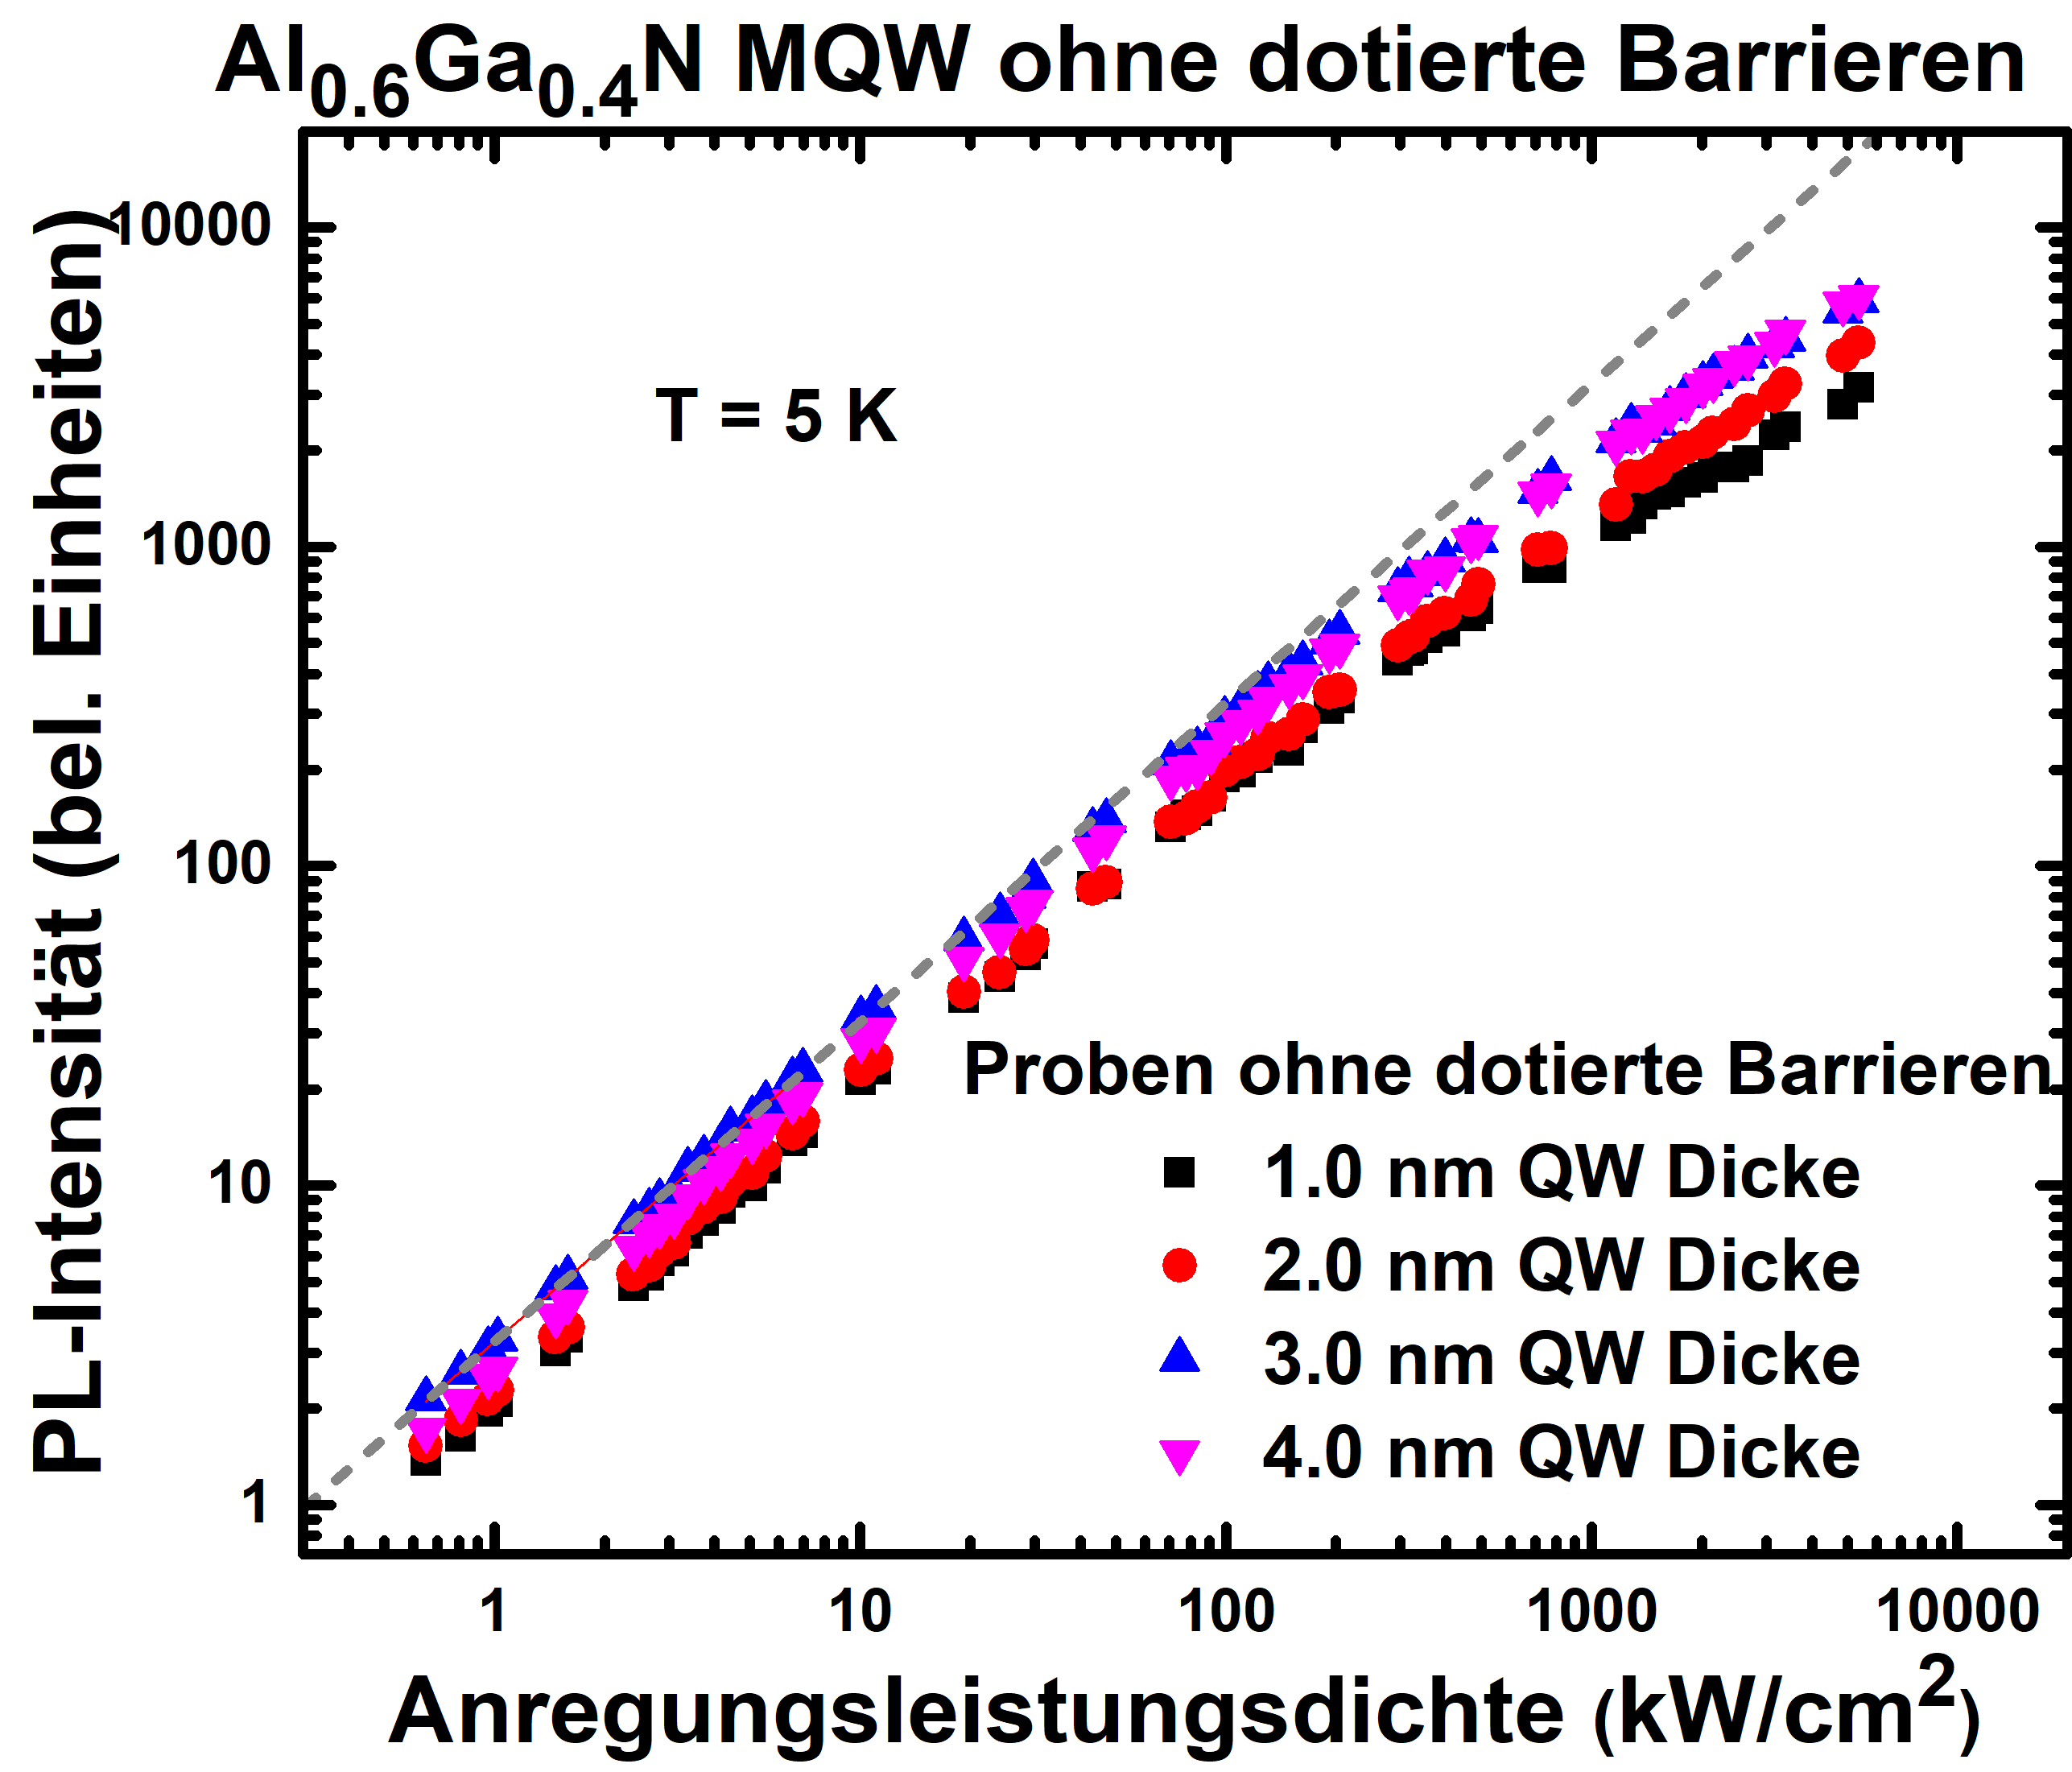
\includegraphics[width=\textwidth]{Bilder/MQWdickenSerie/intTTundotiert.png}
		\caption{Integrierte Intensität in doppeltlogarithmischer Darstellung in Abhängigkeit der Anregungsleistungsdichte bei Tieftemperatur für die Proben mit undotierter Barriere.}
    \label{fig:undotiertint}
  \end{minipage}
	\hfill
  \begin{minipage}[t]{0.49\textwidth}
    \centering
    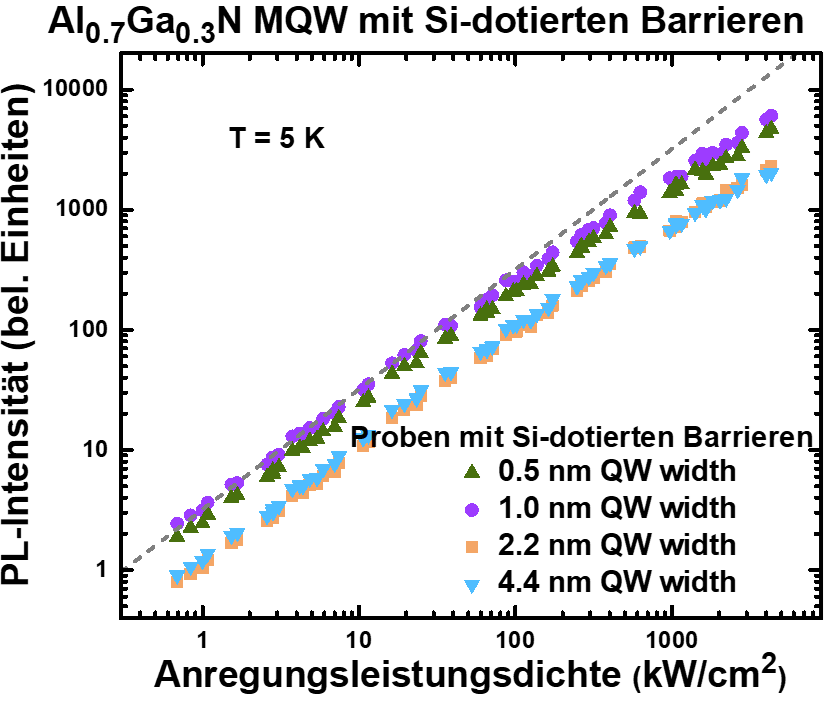
\includegraphics[width=\linewidth]{Bilder/MQWdickenSerie/intTTdotierte.png}
		\caption{Integrierte Intensität in doppeltlogarithmischer Darstellung in Abhängigkeit der Anregungsleistungsdichte bei Tieftemperatur für die Proben mit dotierter Barriere.}
    \label{fig:dotiertint}
  \end{minipage}
\end{figure}
\noindent 
%
Im Bereich geringer Anregungsleistungsdichten zeigt sich für beide Serien eine lineare Steigung (gestrichelte Linie) die mit zunehmender Anregungsleistungsdichte ein nichtlinearen Verlauf annimmt der auf die Auger-Rekombination zurückzuführen ist (siehe Kapitel \ref{chap:auger}).
Die integrierten Intensitäten befinden sich für die Proben mit undotierter Barriere bei Tieftemperatur für alle QW-Dicken auf dem selben Niveau.
Die Proben mit einer QW-Dicke von $3,0 \thinspace nm$ und $4,0 \thinspace nm$ leuchten am hellsten und darauf folgen die Proben mit $2.0 \thinspace nm$ und $1.0 \thinspace nm$  QW-Dicke. Die Unterschiede sind aber marginal und im Rahmen der Streuung, die durch die unterschiedlichen Fokussierungen und Position im PL-Aufbau zu erwarten sind. Gleiches gilt für die Proben mit dotierter Barriere. Dort fallen die Proben mit QW-Dicken von $2.2 \thinspace nm$ und $4.4 \thinspace nm$ deutlicher ab, jedoch in einem unbedenklichen Maß.   
\begin{figure}[H]
  \centering
  \begin{minipage}[t]{0.49\textwidth}
    \centering
    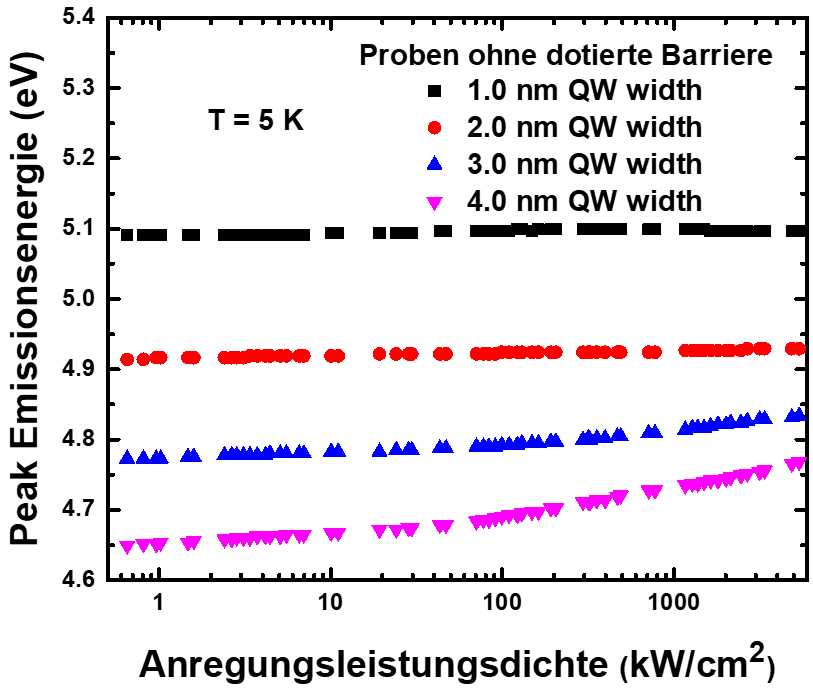
\includegraphics[width=\textwidth]{Bilder/MQWdickenSerie/PeakEnergieUndotiert.png}
		\caption{Peak Emissionsenergie in Abhängigkeit der Anregungsleistungsdichte bei Tieftemperatur der untersuchten MQW-Proben ohne dotierte Barrieren.}
    \label{fig:undotiertpeak}
  \end{minipage}
	\hfill
  \begin{minipage}[t]{0.49\textwidth}
    \centering
    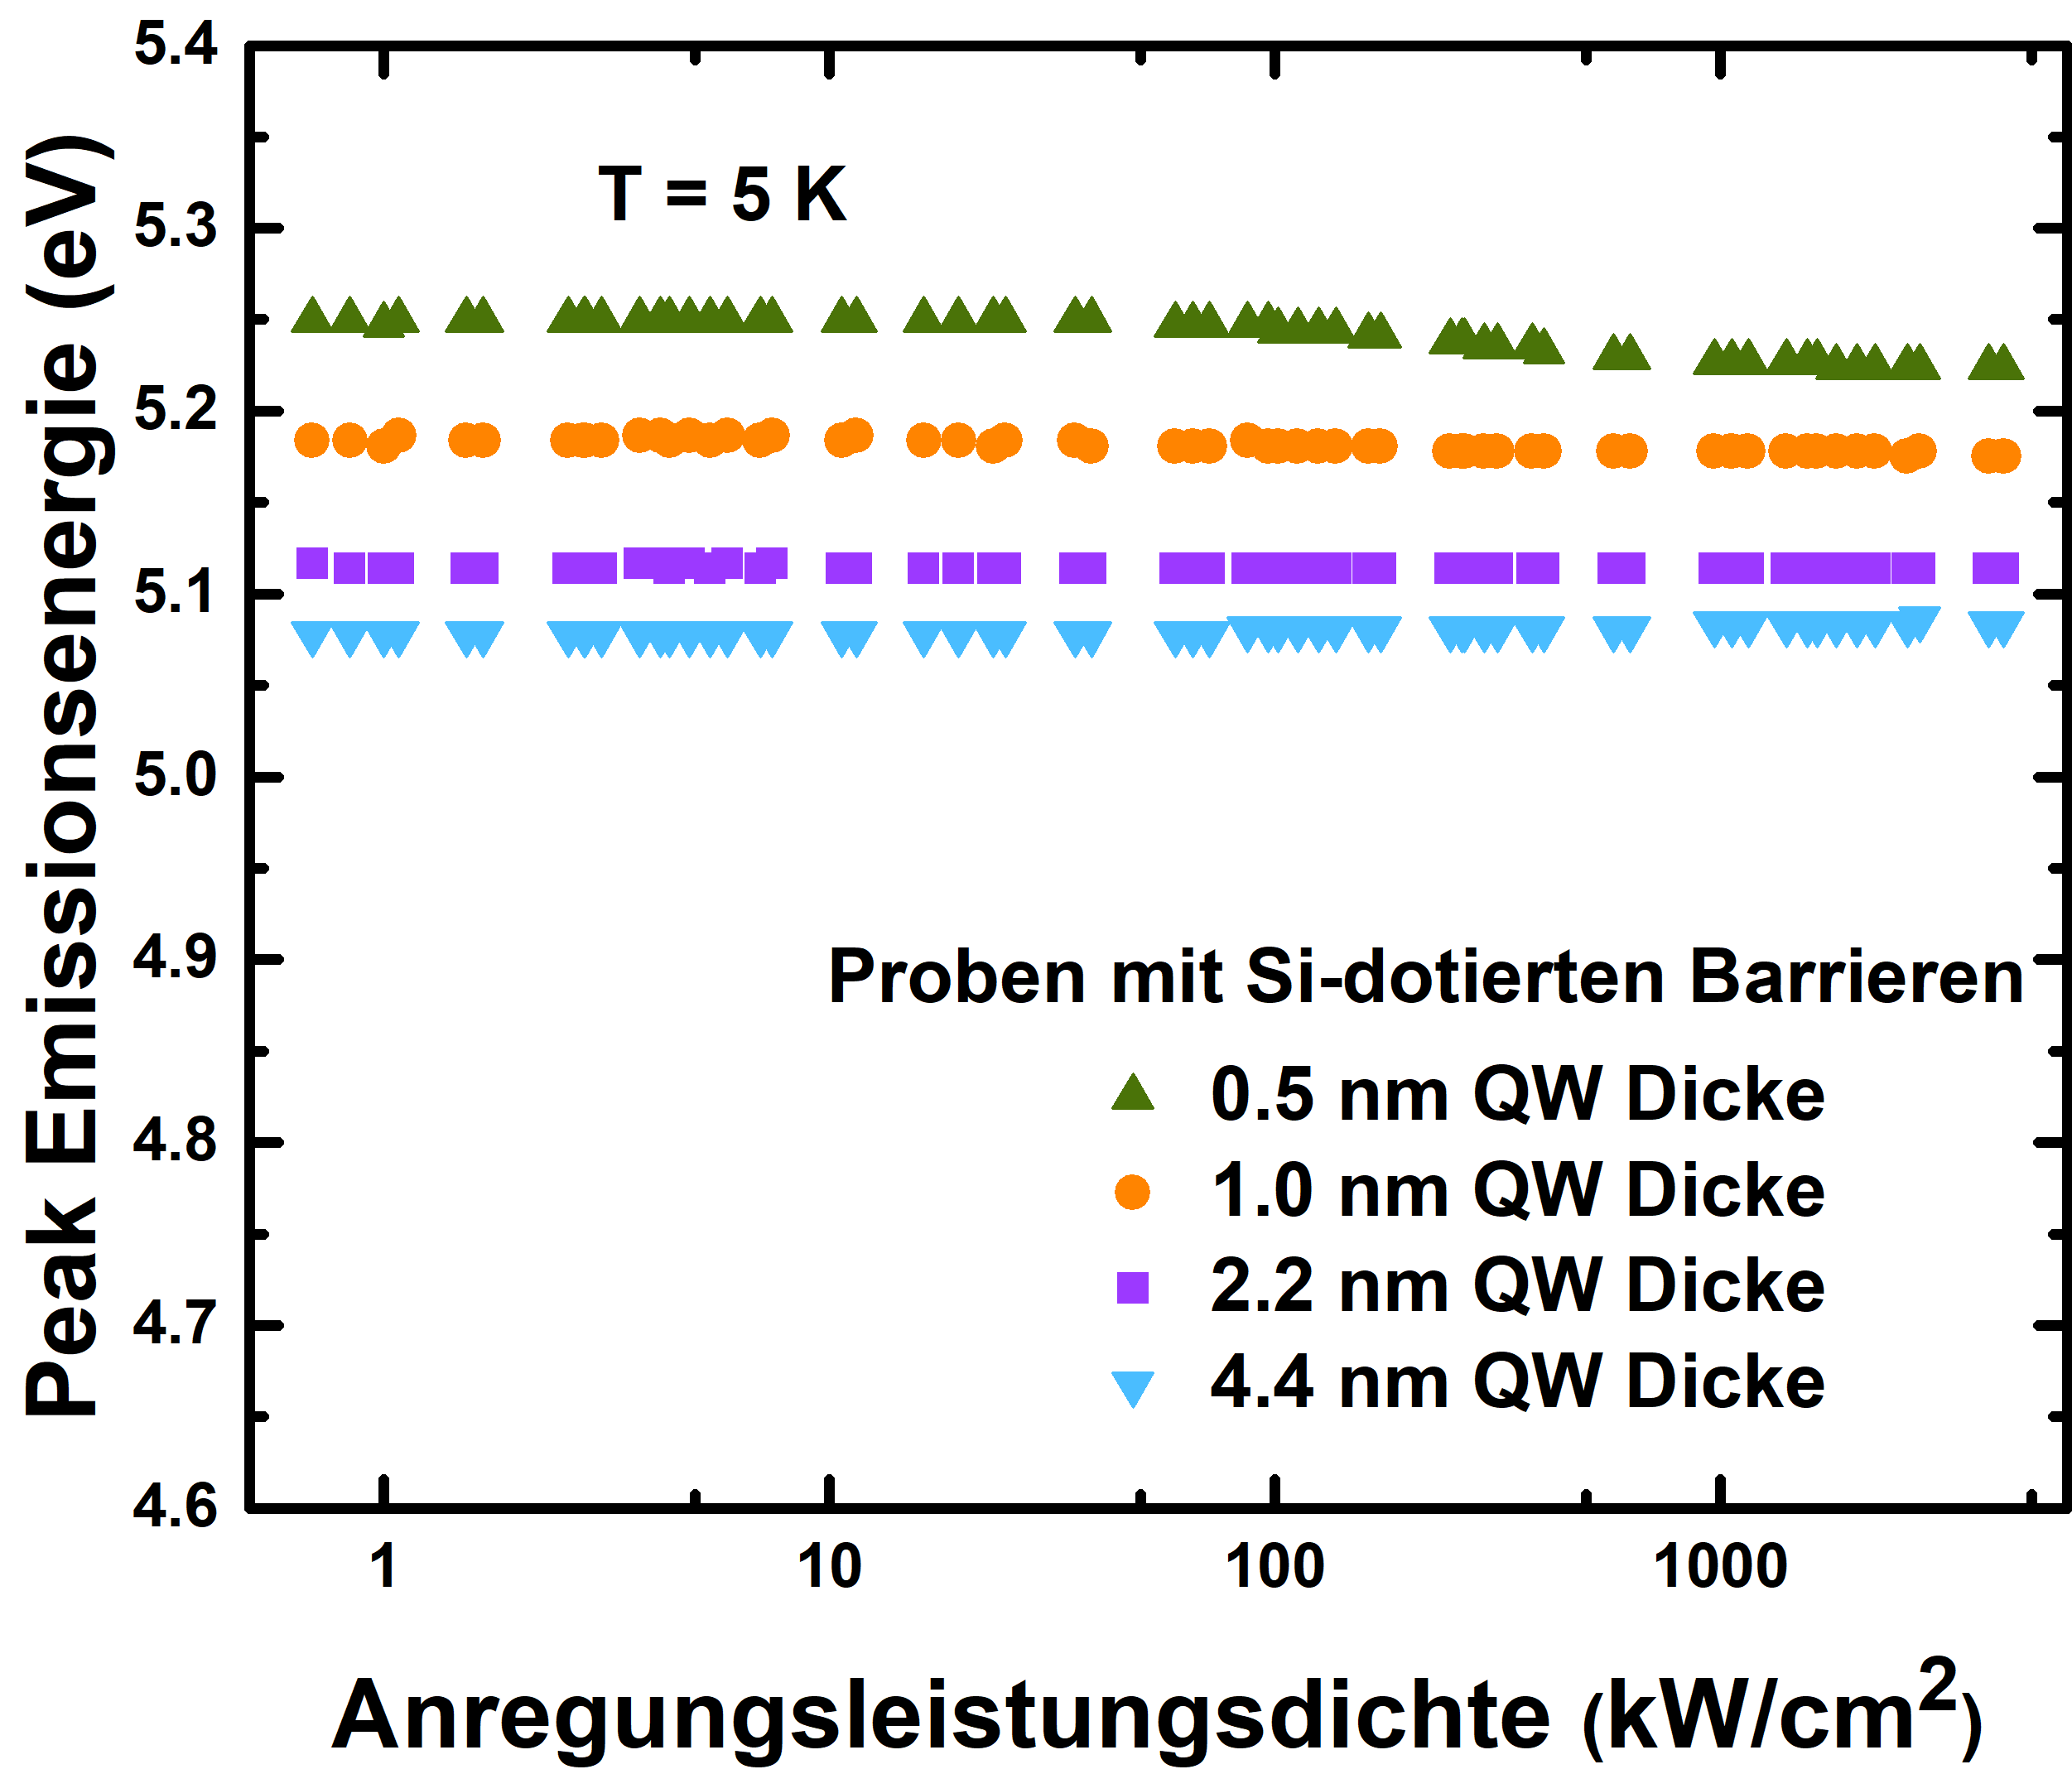
\includegraphics[width=\linewidth]{Bilder/MQWdickenSerie/PeakEnergieDotiert.png}
		\caption{Peak Emissionsenergie in Abhängigkeit der Anregungsleistungsdichte bei Tieftemperatur der untersuchten MQW-Proben mit dotierten Barrieren.}
    \label{fig:dotiertpeak}
  \end{minipage}
\end{figure}
\noindent 
Die Abbildungen \ref{fig:undotiertpeak} und \ref{fig:dotiertpeak} zeigen die Peak-Emissionsenergie des QW in Abhängigkeit der Anregungsleistungsdichte für die Proben mit und un-dotierten Barrieren bei Tieftemperatur. 
\newline
Für die Proben mit undotierten Barrieren ist zu erkennen, dass mit steigender Anregungsleistungsdichte die Emissionsenergie steigt. Der Grund hierfür ist das Screening des QCSE. Dieser Effekt wird größer mit kleiner werdender QW-Dicke, weil mit kleinerer QW-Dicke eine geringere Ladungsträgerdichte im QW notwendig ist, um die Bandverbiegung durch QCSE aufzuheben. 
\newline
So ist die Verschiebung der Peak-Emissionsenergien bei der Probe mit einer QW-Dicke von $5 \thinspace nm$ von $4,65 \thinspace eV$ bei der geringsten Anregungsleistungsdichte zu $4,77 \thinspace eV$ bei der höchsten Anregungsleistungsdichte am stärksten. Die Probe mit einer QW-Dicke von $1 \thinspace nm$ zeigt dagegen keine Verschiebung der Peak-Emissionsenergien. 
\newline
Die Proben mit dotierten Barrieren zeigen dagegen ein anderes Verhalten, so sind die Peak-Emissionsenergien für die Proben mit einer QW-Dicke von 
$1,0 \thinspace nm$, $2,2 \thinspace nm$ und $4,4 \thinspace nm$ nahezu konstant über den ganzen Bereich der Anregungsleistungsdichte, aber die Emissionsenergie der Probe mit der geringsten QW-Dicke von $0,5 \thinspace nm$ verschiebt sich mit steigender Anregungsleistungsdichte hin zu kleineren Energie. Die Gründe für dieses Verhalten sind bisher unklar.
\begin{figure}[H]
  \centering
  \begin{minipage}[t]{0.49\textwidth}
    \centering
    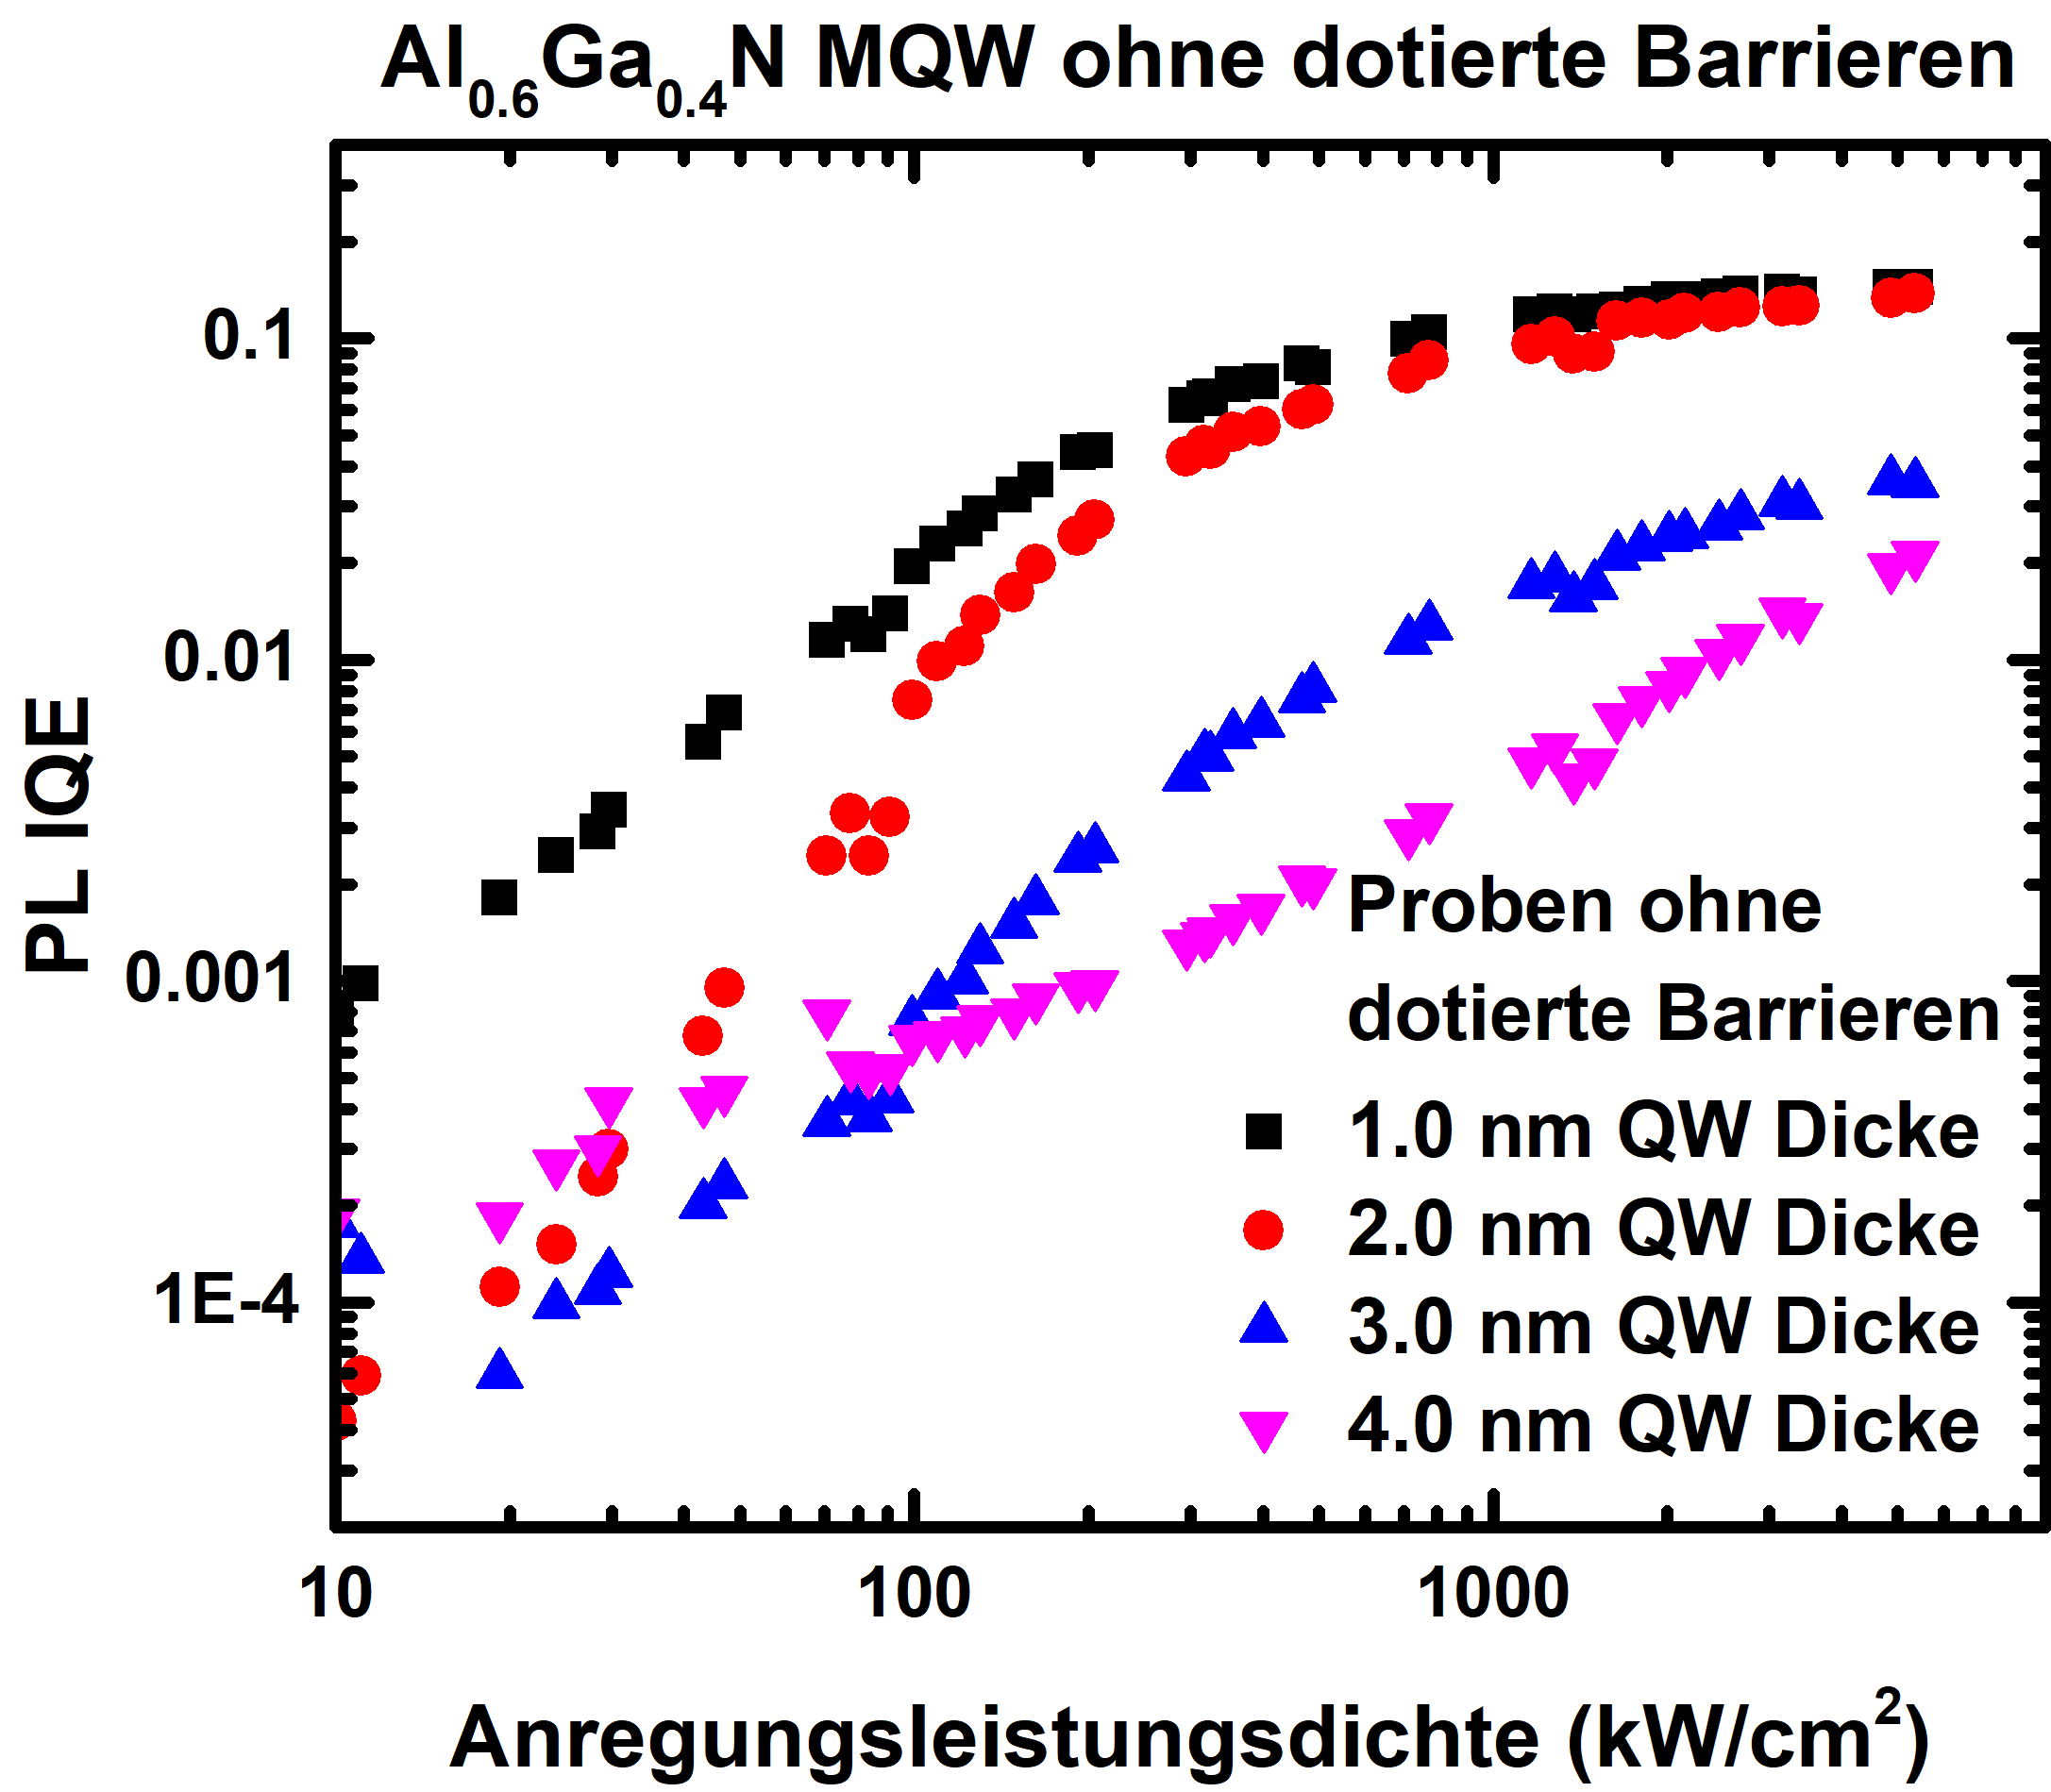
\includegraphics[width=\textwidth]{Bilder/MQWdickenSerie/IQEundotiert.png}
		\caption{IQE in Abhängigkeit der Anregungsleistungsdichte bei Raumtemperatur der untersuchten MQW-Proben ohne dotierte Barrieren.}
    \label{fig:undotiertIQE}
  \end{minipage}
	\hfill
  \begin{minipage}[t]{0.49\textwidth}
    \centering
    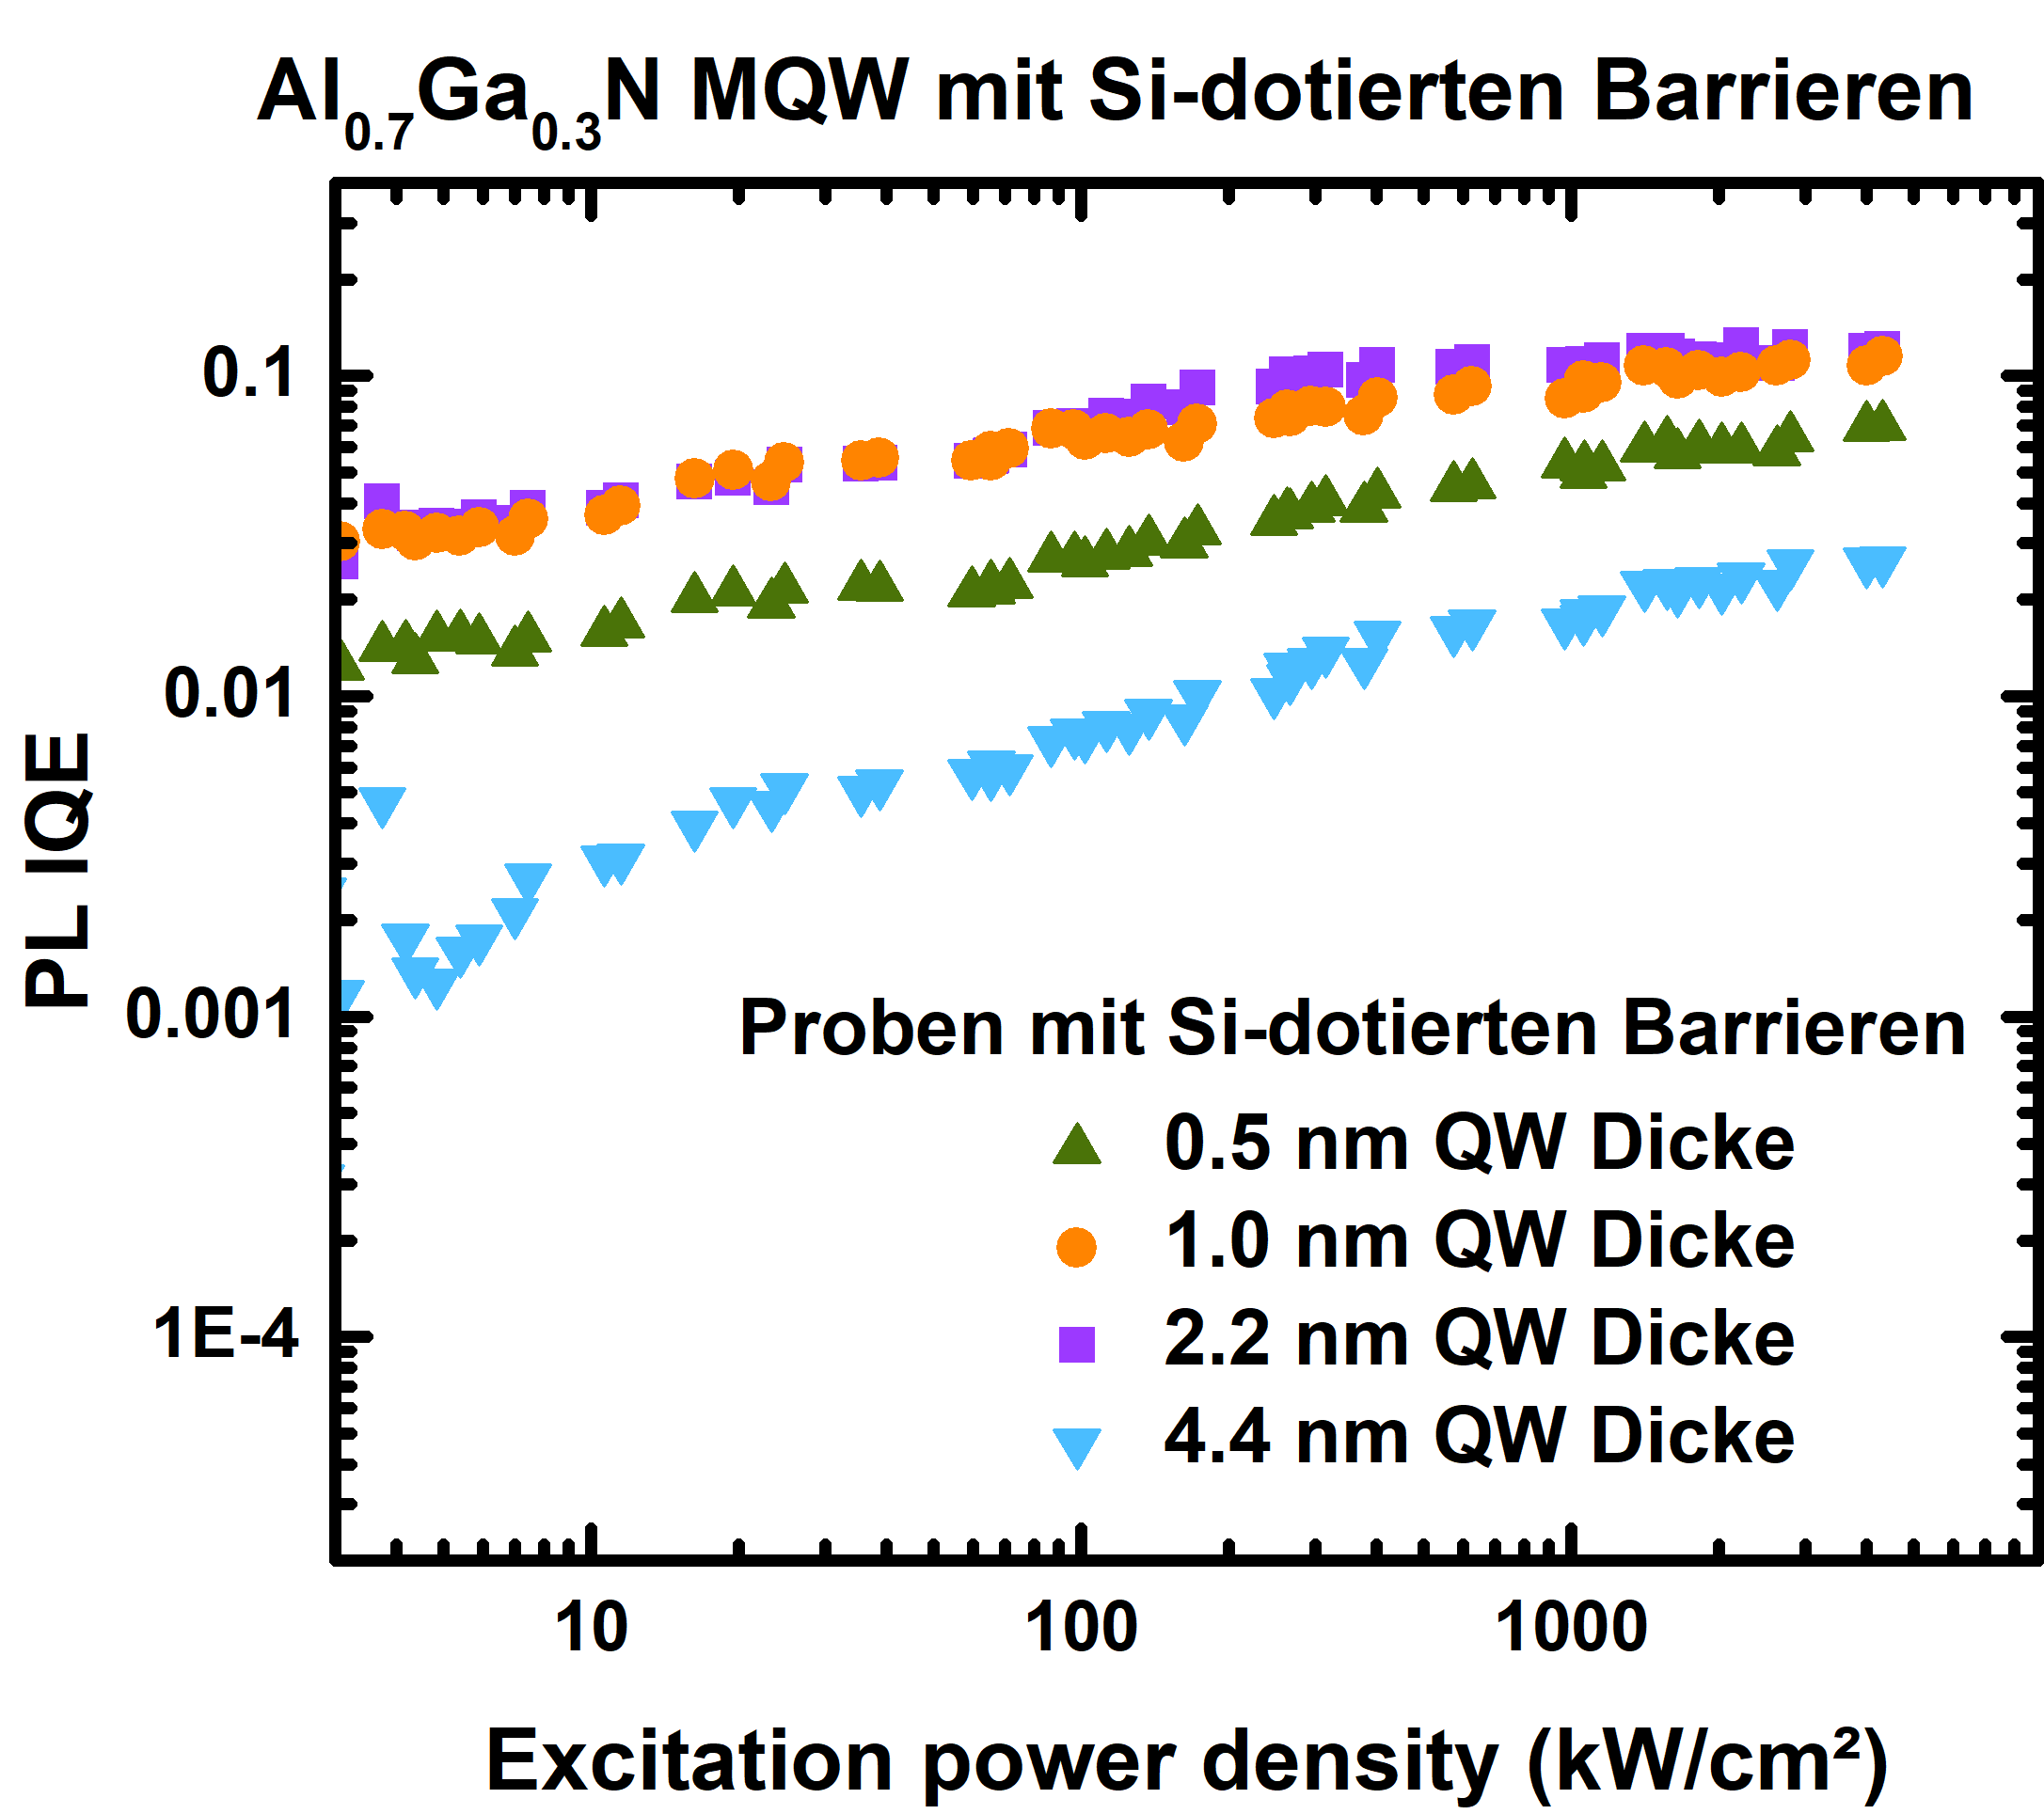
\includegraphics[width=\linewidth]{Bilder/MQWdickenSerie/IQEdotiert.png}
		\caption{IQE in Abhängigkeit der Anregungsleistungsdichte bei Raumtemperatur der untersuchten MQW-Proben.}
    \label{fig:dotiertIQE}
  \end{minipage}
\end{figure}
\noindent 
Die Ergebnisse der IQE bei Raumtemperatur für die Proben ohne und mit dotierten Barrieren sind in den Abbildungen 
\ref{fig:undotiertIQE} und \ref{fig:dotiertIQE} zu sehen. Für beide Probenserien zeigt sich, dass aufgrund des QCSE die IQE für weite QWs 
($3.0 -4.0  nm$) geringer ausfällt und für besonders geringe Dicken ($0.5\thinspace nm$), wahrscheinlich durch den schlechteren Ladungsträgereinschluss, ebenfalls. Die höchste IQE wird für QW-Dicken von $1.0 \thinspace nm- 2.2 \thinspace nm$ gemessen. Die Proben ohne dotierte Barrieren haben eine IQE von ca. $0,145$ bei höchster Anregungsleistungsdichte für die Proben mit QW-Dicken von $1.0 \thinspace nm$ und $2.0\thinspace nm$. 
\newline
Die Proben mit dotierten Barrieren haben eine IQE von ca. $0,121$ bei höchster Anregungsleistungsdichte für die Proben mit QW-Dicken von $1.0 \thinspace nm$ und $2.2\thinspace nm$. Anhand der Ergebnisse für die Proben mit dotierten Barrieren ist zu erkennen, dass die Si-dotierung einen deutlichen Einfluss auf den Verlauf der IQE hat, so ist die Ordinate der IQEs für diese Proben deutlich höher, wie Abbildung \ref{fig:dotiertIQE} zeigt. Die Dotierung führt sichtbar zu höheren IQEs bei geringen Anregungsleistungsdichten die Steigung mit anwachsender Anregungsleistungsdichte ist aber im Vergleich geringer, sodass die IQEs für beide Serien ungefähr den selben Wert einnehmen.

\section{Einfluss der Siliziumdotierung auf die IQE}
Nun soll das ABC-Modell erweitert werden um damit die höhere Ordinate in der IQE für die dotierten Proben zu erklären.
%
\begin{figure}[H]
    \centering
    \begin{minipage}[t]{0.49\linewidth}
        \centering
        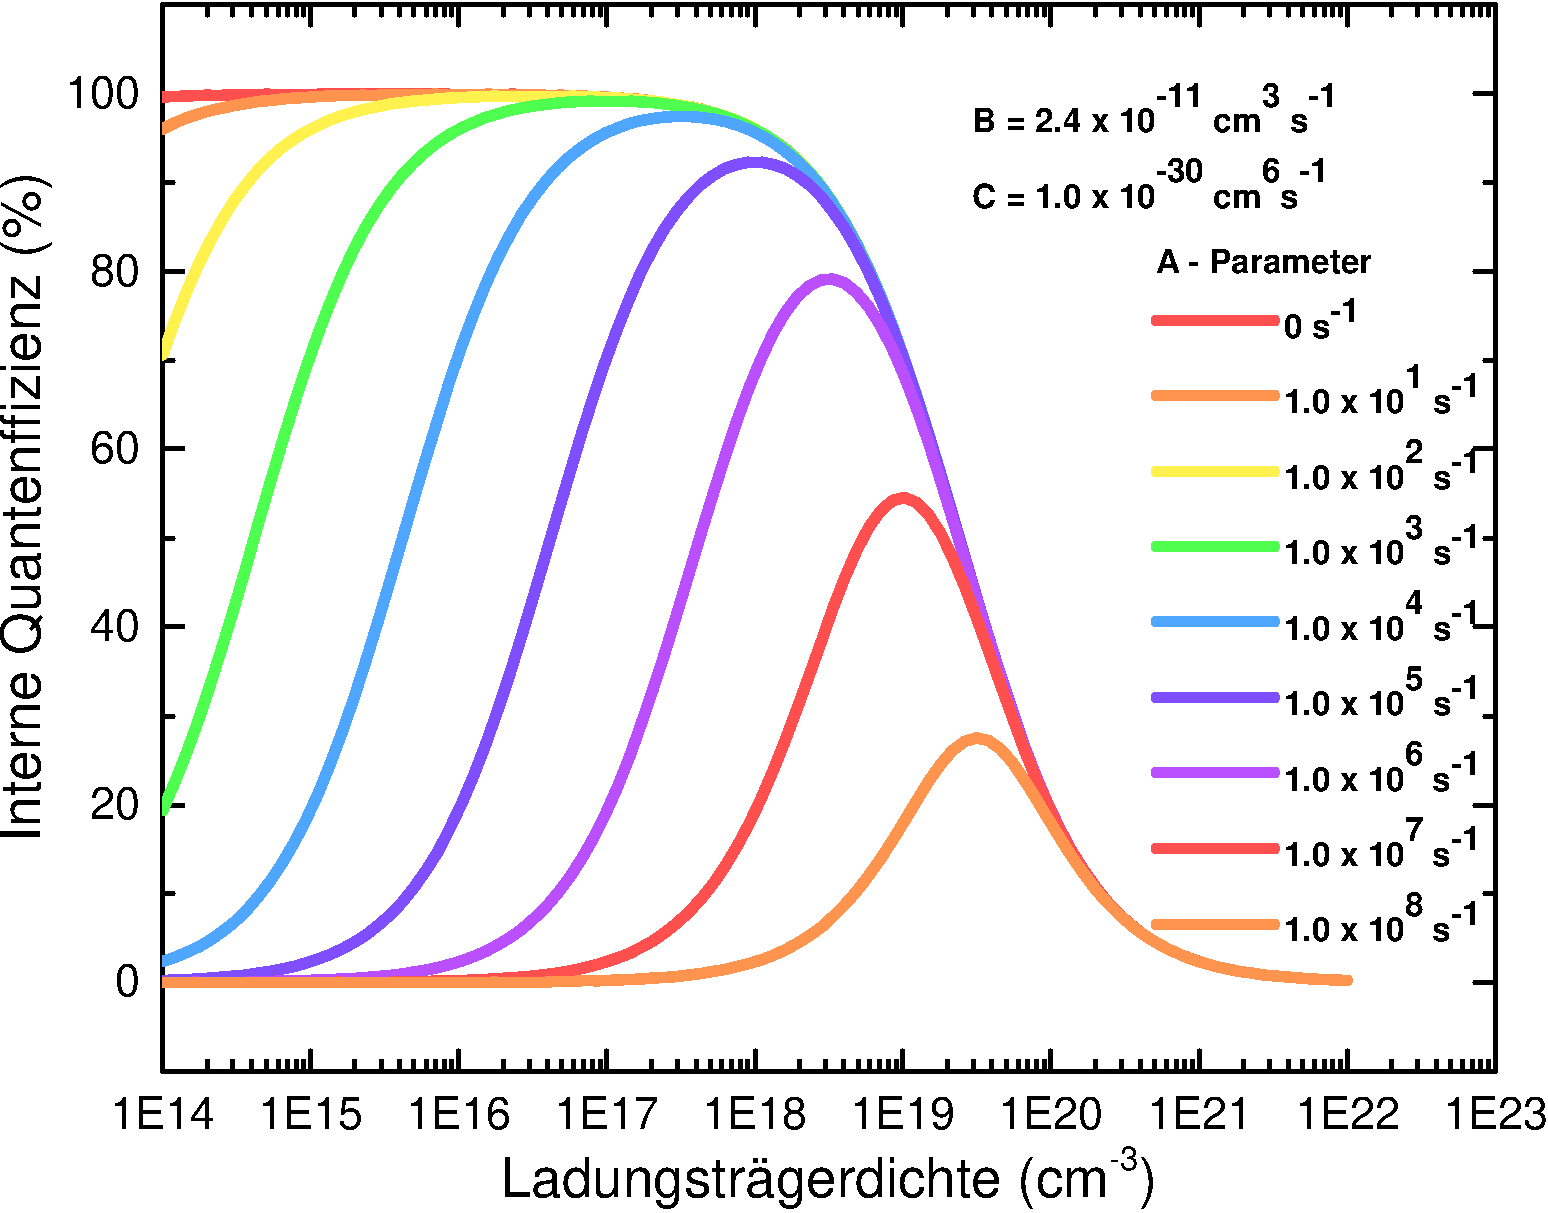
\includegraphics[width=\linewidth]{Bilder/IQEohneDotierungVerschAParams.pdf}
        \caption{Die Grafik zeigt}
        \label{fig:iqenorm}
    \end{minipage}% <- sonst wird hier ein Leerzeichen eingefügt
    \hfill
    \begin{minipage}[t]{0.49\linewidth}
        \centering
        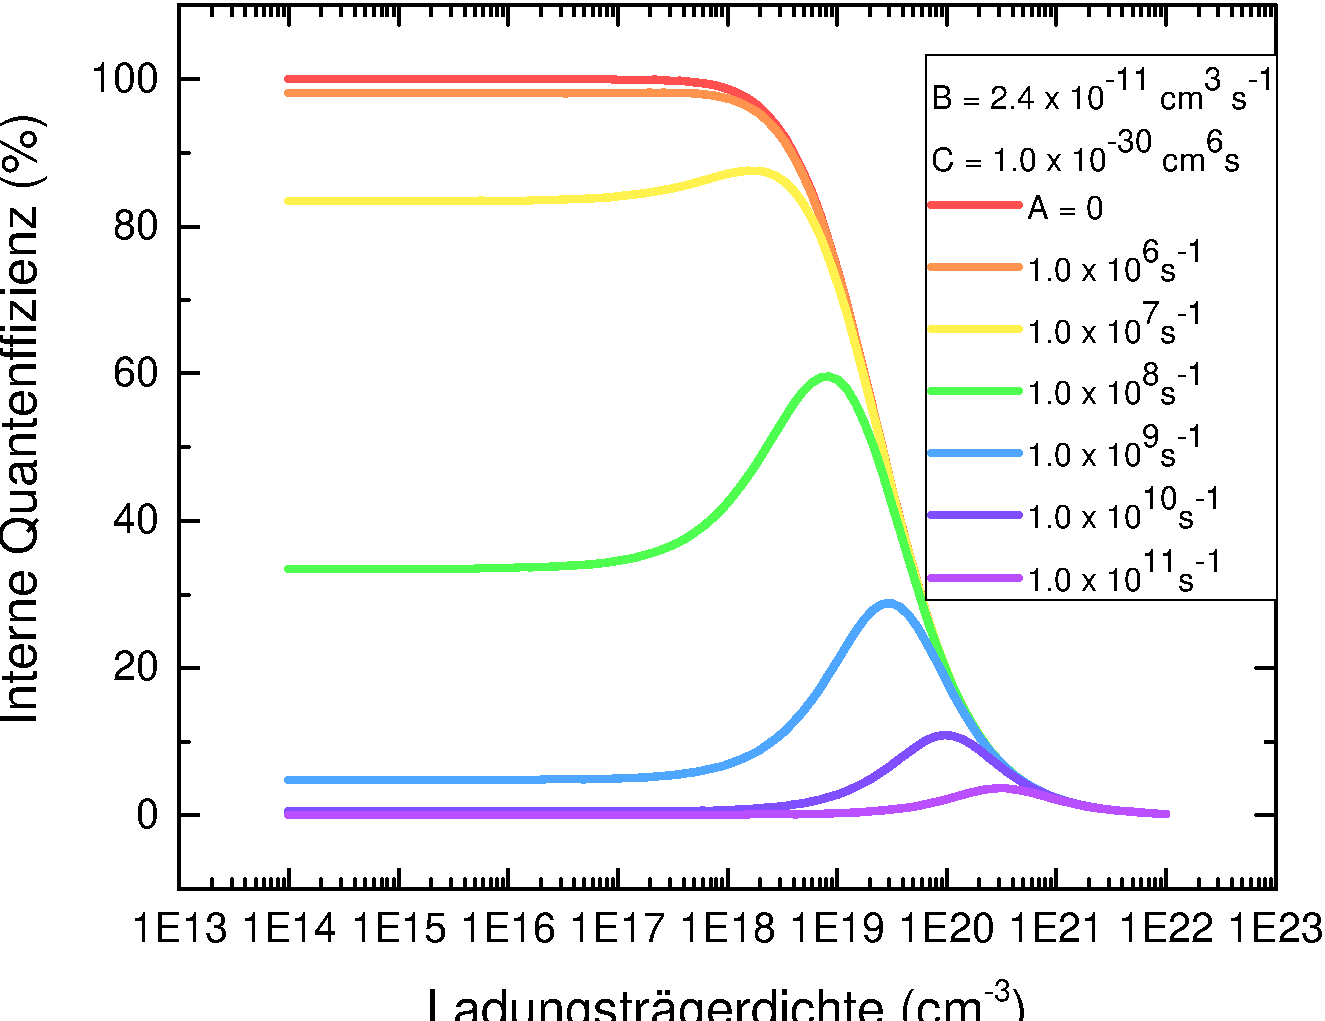
\includegraphics[width=\linewidth]{Bilder/IQEmitDotierungVerschAParams.pdf}
        \caption{Die Grafik zeigt  }
        \label{fig:iqedot}
    \end{minipage}
\end{figure}
\vspace{0.1cm}
\noindent
Das ABC-Modell stellt nur eine Vereinfachung dar und berücksichtigt nicht alle vorkommenden Effekte wie beispielsweise Lokalisierung, Screening durch Ladungsträger und Dotierung. 
Der Effekt der Dotierung spielt dabei eine besonders wichtige Rolle, da eine Silizumdotierung üblich in UV-LEDs ist und einen großen Einfluss hat.
Nach \cite{schub} kann gezeigt werden, dass die Ratengleichungen, mit der Annahme einer Dotierung für die 
die Radiative Rekombination sich ändert und soll nun hergeleitet werden:
\\newline
Jeder dotierte oder undotierte Halbleiter hat zwei Arten von Ladungsträgern, Elektronen und Löcher.
Im Gleichgewicht, bedeutet ohne externe Anregung durch Absorption von Licht oder Injektion von Elektronen, ist das Produkt von Elektronen- und Lochkonzentration eine konstante Größe.
\begin{equation}
    n_0 \cdot p_0 = n_i^2
    \label{eq:constant}
\end{equation}
Hierbei sind $n_0$ und $p_0$ die Elektron- und Lochkonzentration unter Gleichgewichtsbedingung und $n_{i}$ damit die intrinsische Ladungsträgerkonzentration.
Werden zusätzlich die durch Anregung erzeugten Ladungsträger betrachtet, so ist die Gesamtladungsträgerkonzentration gegeben als Summe der Anregungs- und Gleichgewichtsladungsträger. 
\begin{equation}
    n_{ges} = n_0 + n \medspace \text{und} \medspace  p_{ges} = p_0 +  n 
\end{equation}
Hierbei sind $ n$ und $p$ die Anregungsladungsträger. 
Die Anzahl der stattfindenden Rekombination zwischen Elektronen und Löchern sind direkt proportional zur Elektronen-und Ladungsträgerkonzentration, so gilt, $R \propto n \cdot p $. Mit einer Proportionalitätskonstante, wird die Rekombinationsrate pro Zeit und Volumen definiert als
\begin{equation}
    R = - \frac{dn_{ges}}{dt} = - \frac{dp_{ges}}{dt} = B \cdot n_{ges} \cdot p_{ges}
\end{equation}
Weil Elektronen und Löcher bei Anregung paarweise erzeugt werden und verschwinden (durch Rekombination), gilt
\begin{equation}
    \label{eq:gleich}
    n(t) =  p(t)
\end{equation}
Die radiative Rekombinationrate wird dann mit $p_{0} = 0$ und Gleichung \ref{eq:gleich} zu
\begin{align}
\begin{split}
    R_{rad} &= B \cdot (n_0 + n)  \cdot (p_0 + p) ,
    \\
    R_{rad} &= B \cdot (n_0 + n) \cdot (n) ,
    \\
    R_{rad} &= B \cdot n^2 \cdot n \cdot n_0
\end{split}
\end{align}
Dabei beschreibt $n_{0}$ die Ladungsträgerkonzentration durch die Silizumdotierung. 
Somit wird die IQE zu:
\begin{equation}
    IQE = \frac{B \cdot n^2 + B \cdot n \cdot n_{0}}{A \cdot n + B \cdot n^2  + B \cdot n \cdot n_{0}+ C \cdot n^3} 
    \label{eq:dopediqe}
\end{equation}
Und hat einen enormen Einfluss auf die Ordinate, wie in Abb. \ref{fig:iqedot} zu sehen ist.
\section{Ergebnisse der Simulationen}
\begin{figure}[H]
  \centering
  \begin{minipage}[t]{0.49\textwidth}
    \centering
    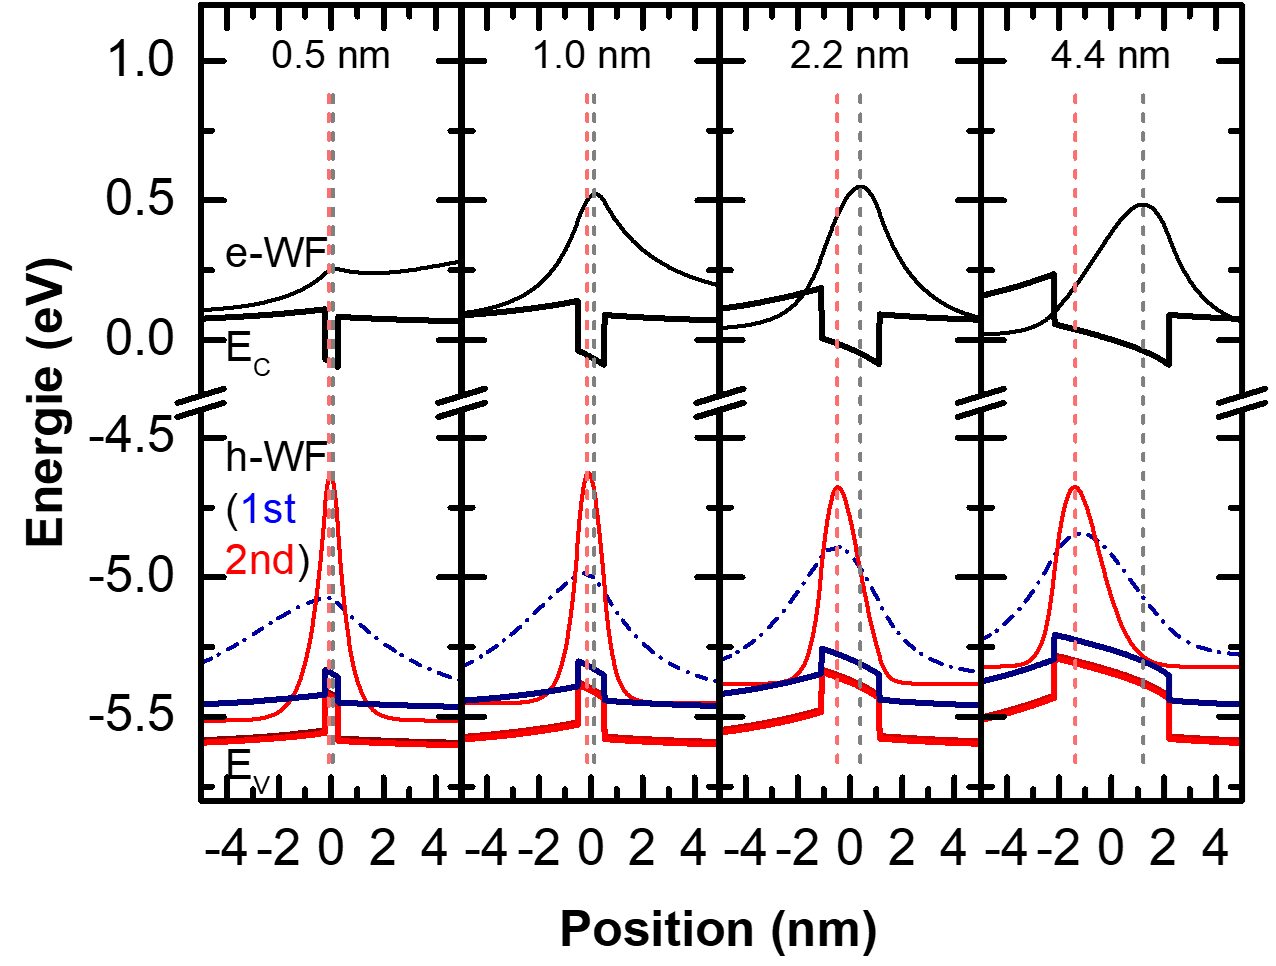
\includegraphics[width=\textwidth]{Bilder/MQWdickenSerie/Simu1.png}
		\caption{Simulation der Elektron- und Lochwellenfunktion im Bändermodell mit QW in einem Bereich von $-4$ bis $4 \thinspace nm$ für verschiedene Dicken. Simulation von Christoph Reich.}
    \label{fig:undotiertSpektrum}
  \end{minipage}
	\hfill
  \begin{minipage}[t]{0.49\textwidth}
    \centering
    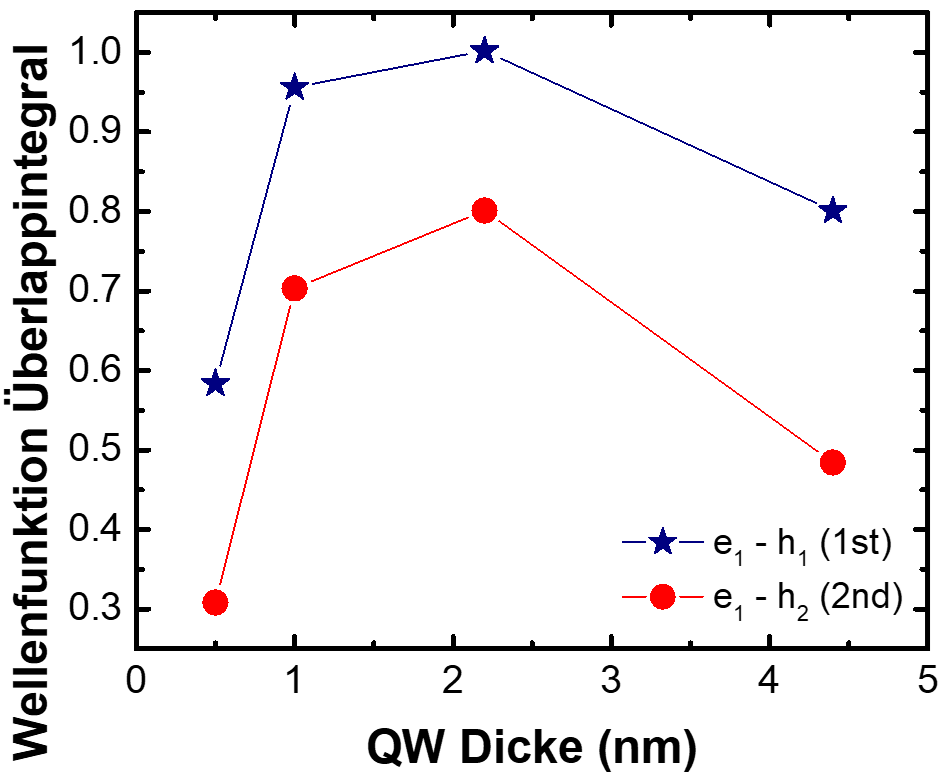
\includegraphics[width=\linewidth]{Bilder/MQWdickenSerie/Simu2.png}
		\caption{Wellenfunktion Überlappintegral in Abhängigkeit der QW-Dicke. Simulation von Christoph Reich.}
    \label{fig:dotiertSpektrum}
  \end{minipage}
\end{figure}
\noindent 
% 
Abbildung und zeigen Modellberechnungen von Christoph Reich basierend auf der k$\cdot$p-Theorie für variierende QW-Dicken. Die Simulation bestätigt, dass für eine QW-Dicke von $0,5 \thinspace nm$ die IQE wegen kleinerem Ladungsträgereinschluss geringer ausfällt und dass durch den QCSE die Separation von Elektron- und Lochwellenfunktion steigt. Dies führt zur Reduktion der strahlenden Rekombinationsrate und bedeutet, dass die IQE für weite QWs geringer ausfällt. Die Simulation bestätigt ebenfalls, dass QW-Dicken zwischen $1.0 \thinspace nm- 2.2 \thinspace nm$ die beste Grundlage für die Verwendung in LEDs darstellen.

\section{Zusammenfassung}

Die Ergebnisse dieses Kapitels zeigen, dass die QW-Dicke einen eindeutigen Einfluss auf die Rekombination und damit auf die IQE hat. Es wurde gezeigt, dass QW-Dicken von $1.0 \thinspace nm- 2.2 \thinspace nm$ die höchsten IQEs liefern. Diese liegen für die Proben mit dotierten und undotierten Barrieren zwischen $0,121$ und $0,145$ und sind damit auf einem ähnlichen Niveau. Die Dotierung führt nur im Bereich geringer Anregungsleistungsdichten zu höheren IQEs. Weiter wurde gezeigt, dass die Emissionsenergien der undotierten Proben durch das Screening des QCSE steigen mit zunehmender Ladungsträgerdichte. Die Proben mit dotierten Barrieren zeigen dagegen ein anderes Verhalten, dessen Ursprung nicht geklärt werden konnte.   